\title{Update to the identification guide to female Alaskan bumble bees and a summary of recent changes to the Alaskan bumble bee fauna}

\subtitle{\doi{10.7299/X7GH9J8D}}

\author{by 
 Derek S.\ Sikes\footnote{University of Alaska Museum, Institute of Arctic Biology, University of Alaska Fairbanks, Fairbanks, Alaska, USA \email{dssikes@alaska.edu}} and
 Jessica J.\ Rykken\footnote{Denali National Park and Preserve, Alaska, USA \email{jessica\_rykken@nps.gov}}
 }

\maketitle

\end{multicols}

\vspace{-1cm}
\begin{center}
 \parbox[t][][s]{14cm}{\section{Summary}
 We summarize numerous recent changes to the taxonomy of the bumble bee fauna of Alaska since \citet{Pampell2010, Pampell2013}, \citet{KochStrange2012} and \citet{Pampelletal2012, Pampelletal2015}. Nine species are now referred to using different names and two new species were described.

 \begin{enumerate}
\item \citet{Williamsetal2014} resulted in the names \textit{Bombus bohemicus}, \textit{Bombus flavidus}, and \textit{Bombus cryptarum} replacing the previous names of \textit{Bombus ashtoni}, \textit{Bombus fernaldae}, and \textit{Bombus moderatus}, respectively. The former three names replace the latter three for all records in Alaska.

\item \citet{Williamsetal2015} elevated \textit{Bombus natvigi} and \textit{Bombus kirbiellus} from invalid as synonyms under \textit{Bombus hyperboreus} and \textit{Bombus balteatus}, respectively, to valid species status. All former records of \textit{B.\ hyperboreus} in Alaska are now \textit{B.\ natvigi}. All former records of \textit{B.\ balteatus} in Alaska are now \textit{B.\ kirbiellus}.

\item A new species, \textit{Bombus kluanensis}, was described by \citet{Williamsetal2016} from Yukon, Canada and Denali National Park and Preserve, Alaska.

\item Since 2017 we consider \textit{Bombus centralis} to be a doubtful member of the Alaskan fauna with all prior records of this species most likely being \textit{Bombus flavifrons}. 

\item \citet{Martinetetal2019} concluded \textit{Bombus sylvicola} is conspecific with \textit{Bombus lapponicus} and established it as a subspecies, thus all Alaskan \textit{Bombus sylvicola} are now \textit{Bombus lapponicus sylvicola}.

\item A new apparently rare species was described from the Alaskan Arctic: \textit{Bombus interacti} by \citet{Martinetetal2019}.

\item Since December 2019 we consider \textit{Bombus suckleyi} to be a doubtful member of the Alaskan fauna with all prior records of this species most likely being \textit{Bombus bohemicus}. 

\item \citet{Ghisbainetal2020} split \textit{Bombus bifarius} into two species and \textit{B.\ bifarius} does not occur in Alaska. All Alaskan \textit{B.\ bifarius} records should be considered \textit{Bombus vancouverensis}.

\item The Alaskan bumble bee fauna now has 22 confirmed species and 1 doubtful species for a possible total of 23 species.

\end{enumerate}
 }
\end{center}

\vspace{4mm}

\begin{multicols}{2}

\section{Introduction}

There has been a considerable increase in interest in pollinators, and specifically bumble bees, across North America. In part, this interest stems from concerns about observed bumble bee declines, especially in relation to effects from climate change, introduced pathogens, and habitat fragmentation \citep{Cameronetal2011, Kerretal2015, Soroyeetal2020}. In Alaska, there has also been interest in basic questions about species diversity, biology, and distribution \citet{KochStrange2012, Kochetal2012, Hattenetal2015, Pampelletal2015, Rykken2015, Rykken2017}. Since these published works there have been some taxonomic name changes, misidentifications discovered, new species described, and synonymies published which we summarize and comment on here to provide a handy reference for ongoing and future work on the Alaskan bee fauna. Numerous records in \href{https://www.gbif.org/}{GBIF.org} of Alaskan \textit{Bombus} exist under old taxonomic concepts or are misidentifications so such public data should be corrected or subsampled before use.

We have updated the color guide of \citet{Pampell2013} with these corrections and have made changes to the colors of some species figured in the guide to better match Alaskan populations. Note that identification of many species cannot be confirmed by color alone; there are other microscopic characters that may need examination (like malar length), so we strongly recommend this guide be used in conjunction with the \citet{Williamsetal2014} field guide. We also recommend the free PDF guide to bumble bees of the western states by \citet{Kochetal2012}. Color can vary within species (especially on tergites) and our updated guide shows primarily the most common conditions. Color is best observed on clean and dry specimens; it is very difficult to identify bumble bees with matted, dirty hairs. We have marked rarely collected species, those with fewer than 40 Alaskan specimens known to us, with an asterisk in the guide. A review of Alaskan \textit{Bombus} species with state conservation status assessments was recently completed by the Alaska Center for Conservation Science and can be found online (\url{https://accs.uaa.alaska.edu/wildlife/pollinator-diversity/}).

This guide is for female bumble bees. The guide can help for male identification, but males can show a higher degree of variability than females. Females have six visible abdominal (metasomal) segments called tergites, stingers, antennae with 10 flagellomeres, and their mandibles are wide apically and scoop-like. Males have seven visible tergites with the tip of their abdomen blunt and lacking a stinger, have antennae with 11 flagellomeres, and male mandibles are narrow and notably bearded.  

\section{Results}

\setcounter{subsection}{1}
\renewcommand\thesubsection{\arabic{section}}

\subsection{1) Replacement of the names \textit{Bombus ashtoni}, \textit{Bombus fernaldae}, and \textit{Bombus moderatus} by \textit{Bombus bohemicus}, \textit{Bombus flavidus}, and \textit{Bombus cryptarum}}

\citet{Williamsetal2014} resulted in the replacement of the names for three Alaskan species, \textit{Bombus ashtoni}, \textit{Bombus fernaldae}, and \textit{Bombus moderatus} by \textit{Bombus bohemicus}, \textit{Bombus flavidus}, and \textit{Bombus cryptarum}, respectively. The latter three names replace the former three for all records in Alaska. Details on the justifications for these changes can be found in \citet{Williamsetal2014} and the online catalog of \citet{Williams2020}, which cites \citet{Cameronetal2007} as justification for the first two. We have updated the names in the color guide accordingly (Figure \ref{color_guide}).

\subsection{2) Replacement of the names \textit{Bombus hyperboreus} and \textit{Bombus balteatus} by \textit{Bombus natvigi} and \textit{Bombus kirbiellus}}

\citet{Williamsetal2015} elevated \textit{Bombus natvigi} and \textit{Bombus kirbiellus} from invalid as synonyms under \textit{Bombus hyperboreus} and \textit{Bombus balteatus}, respectively, to valid species status. This conclusion was justified based on genetic data that split the former Holarctic species into separate Palearctic and Nearctic species. All former records of \textit{B.\ hyperboreus} in Alaska are now \textit{B.\ natvigi}. All former records of \textit{B.\ balteatus} in Alaska are now \textit{B.\ kirbiellus}. We have updated the names in the color guide accordingly (Figure \ref{color_guide}).

\subsection{3) Discovery of new species in Denali National Park, Alaska---\textit{Bombus kluanensis}}

\textit{Bombus kluanensis}, recently described by \citet{Williamsetal2016}, is currently known in Alaska only from Denali National Park and Preserve. In the park, it has been collected in several alpine tundra sites. Many more specimens have also been collected in the Kluane region and St.\ Elias Range in Yukon, Canada. It is very likely that \textit{B.\ kluanensis} occurs in Wrangell-St.\ Elias National Park and Preserve, which encompasses the eastern end of the Alaska Range and the western end of the St.\ Elias Range. However, a brief survey of alpine tundra sites off the Nabesna Road in Wrangell-St.\ Elias in 2018 yielded no \textit{B.\ kluanensis} specimens. Further surveys are needed for this species to fully document its range in Alaska.

\end{multicols}
\begin{figure}[H]
\begin{center}
%\vspace{2mm}
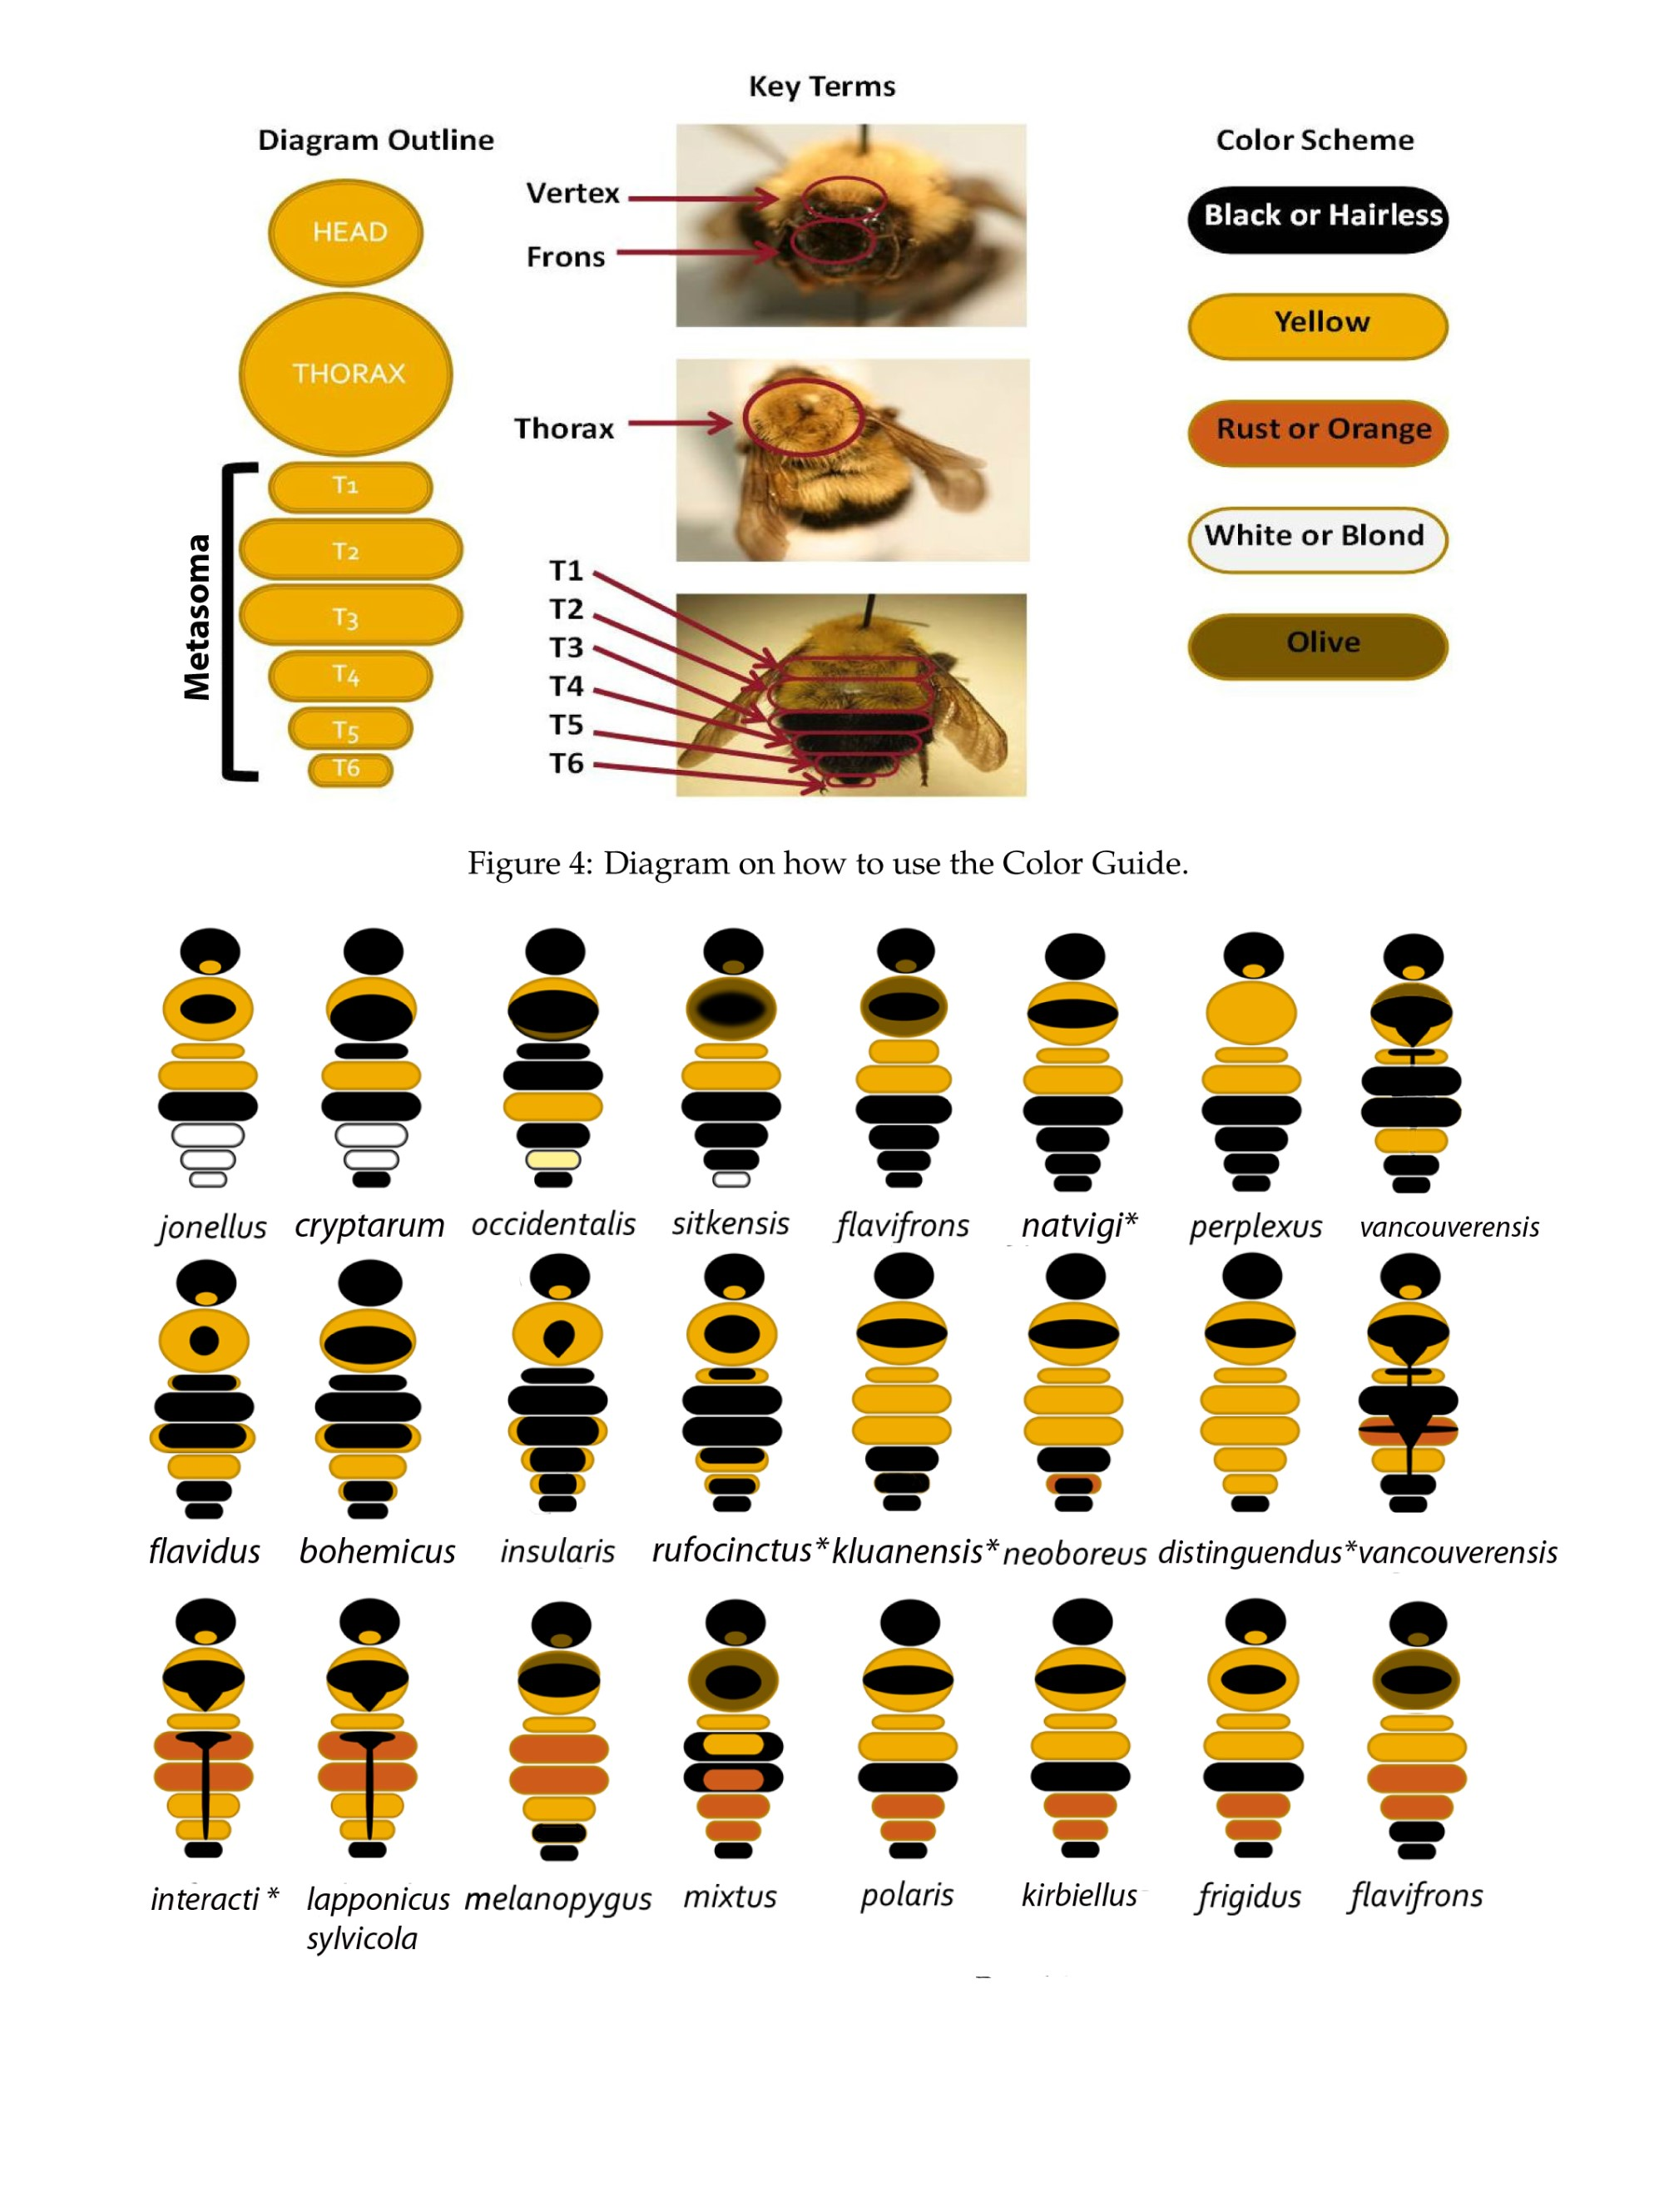
\includegraphics[width=\textwidth]{img/bumblebee_guide.jpg}
\caption{Color guide to common interior bumblebees of Alaska based on that of \citet{Pampell2010} with names and some colors updated. Rarely collected species, those with fewer than 40 Alaskan specimens known to us, are marked with an asterisk.}
\label{color_guide}
\end{center}
\end{figure} 
\begin{multicols}{2}

\subsection{4) \textit{Bombus centralis} and \textit{Bombus flavifrons} misidentification}

In 2017 we discovered and corrected a large misidentification problem that had occurred between the species \textit{Bombus centralis} and \textit{Bombus flavifrons}. This involved 3,313 specimens in the University of Alaska Museum that had been identified as \textit{B.\ centralis} and cited as such in \citet{Pampell2010} and \citet{Pampelletal2015}, but subsequent examination by the first author determined them to be \textit{B.\ flavifrons}. The cause of this problem stemmed from the Alaska color guide \citep{Pampell2013}. In that guide there was only one color form (the non-orange) for \textit{B.\ flavifrons}. However, \textit{B.\ flavifrons} has an orange color form that is almost identical to \textit{B.\ centralis} \citep{Williamsetal2014}. In Alaska, we have found both color forms occurring in the same area. We have updated the guide with this other form added and removed \textit{B.\ centralis} (Figure \ref{color_guide}). This case demonstrates the importance of not relying only on single color patterns for bumble bee identification and stresses the importance of archiving specimens that allow verification of identifications.

\begin{figure}[H]
\begin{center}
\vspace{2mm}
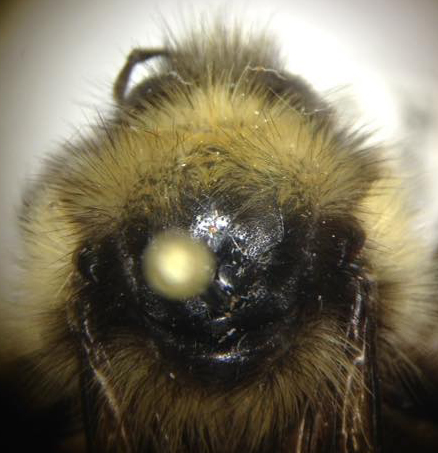
\includegraphics[width=\textwidth]{img/bumblebee_guide_Bombus_flavifrons.jpg}
\caption{Image of \textit{B.\ flavifrons} showing the black hairs intermixed with yellow in the anterior band. \textit{Bombus centralis} has only yellow hairs with no black hairs intermixed.}
\label{B_flavifrons}
\end{center}
\end{figure}

The anterior band of yellow hairs on the thorax differs in color between these species. \textit{Bombus flavifrons} has black hairs mixed among the yellow hairs (Figure \ref{B_flavifrons}) while \textit{B.\ centralis} has only yellow hairs (although we have no authoritatively identified specimens of \textit{B.\ centralis} in the University of Alaska Museum Insect Collection (\acr{UAM})). Males are harder to distinguish because they have far fewer black hairs in the anterior region and some appear to lack black hairs entirely in that region.

\citet{Sikesetal2017} \acr{DNA} barcoded two \acr{UAM} \textit{B.\ centralis} specimens which fell into a \acr{BIN} (Barcode Index Numbers \citep{RatnasinghamHebert2013}) with over 110 \textit{B.\ flavifrons} specimens (\BIN{BOLD:ACE3465}). After having confirmed the specimens had the diagnostic black hairs of \textit{B.\ flavifrons} we edited the records of these two specimens in \acr{BOLD} (Barcode of Life Data System \citep{RatnasinghamHebert2007}) to correct their identifications to \textit{B.\ flavifrons}. These two species are each other’s nearest neighbors in \acr{BOLD} with a genetic distance of only 1.12\%.

\citet{Williamsetal2014} includes a small number of records of \textit{B.\ centralis} in Alaska. Presumably these are records that were confirmed by the authors so this species may belong on the Alaskan list---but if so, it is apparently quite rare. We consider its presence in Alaska doubtful and have not included it on our list (Table \ref{Bombustable}).

\subsection{5) \textit{Bombus sylvicola} in Alaska is now \textit{Bombus lapponicus sylvicola}}

\citet{Martinetetal2019} concluded \textit{Bombus sylvicola} is conspecific with \textit{Bombus lapponicus} and established it as a subspecies. Thus, all \textit{Bombus sylvicola} are now \textit{Bombus lapponicus sylvicola}. The integrative taxonomic research described below for \textit{B.\ interacti} led to this seemingly well-founded conclusion. 

\subsection{6) New, apparently rare, Arctic species---\textit{Bombus interacti} Martinet, Brasero \& Rasmont, 2019}

A new, currently rare, and potentially difficult to identify \textit{Bombus} species was described from the Toolik Field Station in the Alaskan Arctic: \textit{Bombus interacti} by \citet{Martinetetal2019}. \citet{Martinetetal2019} wrote regarding morphological diagnosis of this new species: 

\begin{quotation}
\textit{Bombus interacti} males differed from \textit{B.\ sylvicola} in the pubescence of the tibia, which is hairier in \textit{B.\ sylvicola}. No difference in the structures of the genitalia was detected. Females of \textit{B.\ interacti} differed from \textit{B.\ sylvicola} in the face clypeus coloration: black with intermixed dark yellow hair in \textit{B.\ interacti} and yellow in \textit{B.\ sylvicola}. Besides, the density of pubescence of tergite 5 is higher in \textit{B.\ interacti} and the yellow coloration of the collar does not reach the bases of the legs.
\end{quotation}

\end{multicols}
\begin{center}
\begin{longtable}{rl}

\caption{Twenty-four species of \textit{Bombus} recorded from Alaska based on 34,145 catalog records with the number of records indicated, with links to those records provided through the numbers of records. Records are a mix of specimen and literature records.}\label{Bombustable}\\

\hline
\\[-1.0em]
\hline
\\[-1.0em]
\bf{Record Count} & \bf{\acr{Species}} \\
\hline
\\[-1.0em]
\endfirsthead

\hline
\bf{Record Count} & \bf{\acr{Species}} \\
\hline
\endhead

\multicolumn{2}{c}{\textit{Continued on next page\ldots{}}}\\
\hline
\endfoot

\hline
\\[-1.0em]
\hline
\endlastfoot

\href{https://arctos.database.museum/SpecimenResults.cfm?state_prov=Alaska&scientific_name=Bombus&scientific_name_scope=currentID&species=NOTNULL&taxa_formula=A&formatted_scientific_name==%3Ci%3EBombus%20flavifrons%3C%2Fi%3E%20Cresson%2C%201863}{5,310} & \textit{Bombus flavifrons} Cresson, 1863\\
\href{https://arctos.database.museum/SpecimenResults.cfm?state_prov=Alaska&scientific_name=Bombus&scientific_name_scope=currentID&species=NOTNULL&taxa_formula=A&formatted_scientific_name==%3Ci%3EBombus%20jonellus%3C%2Fi%3E%20(Kirby%2C%201802)}{4,252} & \textit{Bombus jonellus} (Kirby, 1802)\\
\href{https://arctos.database.museum/SpecimenResults.cfm?state_prov=Alaska&scientific_name=Bombus&scientific_name_scope=currentID&species=NOTNULL&taxa_formula=A&formatted_scientific_name==%3Ci%3EBombus%20lapponicus%20sylvicola%3C%2Fi%3E%20Kirby%2C%201837}{4,194} & \textit{Bombus lapponicus sylvicola} Kirby, 1837\\
\href{https://arctos.database.museum/SpecimenResults.cfm?state_prov=Alaska&scientific_name=Bombus&scientific_name_scope=currentID&species=NOTNULL&taxa_formula=A&formatted_scientific_name==%3Ci%3EBombus%20frigidus%3C%2Fi%3E%20Smith%2C%201854}{3,960} & \textit{Bombus frigidus} Smith, 1854\\
\href{https://arctos.database.museum/SpecimenResults.cfm?state_prov=Alaska&scientific_name=Bombus&scientific_name_scope=currentID&species=NOTNULL&taxa_formula=A&formatted_scientific_name==Bombus%20vancouverensis}{3,632} & \textit{Bombus vancouverensis}  Cresson, 1878\\
\href{https://arctos.database.museum/SpecimenResults.cfm?state_prov=Alaska&scientific_name=Bombus&scientific_name_scope=currentID&species=NOTNULL&taxa_formula=A&formatted_scientific_name==%3Ci%3EBombus%20mixtus%3C%2Fi%3E%20Cresson%2C%201878}{3,442} & \textit{Bombus mixtus} Cresson, 1878\\
\href{https://arctos.database.museum/SpecimenResults.cfm?state_prov=Alaska&scientific_name=Bombus&scientific_name_scope=currentID&species=NOTNULL&taxa_formula=A&formatted_scientific_name==%3Ci%3EBombus%20occidentalis%3C%2Fi%3E%20Greene%2C%201858}{2,744} & \textit{Bombus occidentalis} Greene, 1858\\
\href{https://arctos.database.museum/SpecimenResults.cfm?state_prov=Alaska&scientific_name=Bombus&scientific_name_scope=currentID&species=NOTNULL&taxa_formula=A&formatted_scientific_name==%3Ci%3EBombus%20melanopygus%3C%2Fi%3E%20Nylander%2C%201848}{1,572} & \textit{Bombus melanopygus} Nylander, 1848\\
\href{https://arctos.database.museum/SpecimenResults.cfm?state_prov=Alaska&scientific_name=Bombus&scientific_name_scope=currentID&species=NOTNULL&taxa_formula=A&formatted_scientific_name==%3Ci%3EBombus%20perplexus%3C%2Fi%3E%20Cresson%2C%201863}{1,553} & \textit{Bombus perplexus} Cresson, 1863\\
\href{https://arctos.database.museum/SpecimenResults.cfm?state_prov=Alaska&scientific_name=Bombus&scientific_name_scope=currentID&species=NOTNULL&taxa_formula=A&formatted_scientific_name==%3Ci%3EBombus%20cryptarum%3C%2Fi%3E%20(Fabricius%2C%201775)}{997} & \textit{Bombus cryptarum} (Fabricius, 1775)\\
\href{https://arctos.database.museum/SpecimenResults.cfm?state_prov=Alaska&scientific_name=Bombus&scientific_name_scope=currentID&species=NOTNULL&taxa_formula=A&formatted_scientific_name==%3Ci%3EBombus%20insularis%3C%2Fi%3E%20(Smith%2C%201861)}{470} & \textit{Bombus insularis} (Smith, 1861)\\
\href{https://arctos.database.museum/SpecimenResults.cfm?state_prov=Alaska&scientific_name=Bombus&scientific_name_scope=currentID&species=NOTNULL&taxa_formula=A&formatted_scientific_name==%3Ci%3EBombus%20kirbiellus%3C%2Fi%3E%20Curtis%2C%201835}{439} & \textit{Bombus kirbiellus} Curtis, 1835\\
\href{https://arctos.database.museum/SpecimenResults.cfm?state_prov=Alaska&scientific_name=Bombus&scientific_name_scope=currentID&species=NOTNULL&taxa_formula=A&formatted_scientific_name==%3Ci%3EBombus%20flavidus%3C%2Fi%3E%20Eversmann%2C%201852}{389} & \textit{Bombus flavidus} Eversmann, 1852\\
\href{https://arctos.database.museum/SpecimenResults.cfm?state_prov=Alaska&scientific_name=Bombus&scientific_name_scope=currentID&species=NOTNULL&taxa_formula=A&formatted_scientific_name==%3Ci%3EBombus%20polaris%3C%2Fi%3E%20Curtis%2C%201835}{322} & \textit{Bombus polaris} Curtis, 1835\\
\href{https://arctos.database.museum/SpecimenResults.cfm?state_prov=Alaska&scientific_name=Bombus&scientific_name_scope=currentID&species=NOTNULL&taxa_formula=A&formatted_scientific_name==%3Ci%3EBombus%20bohemicus%3C%2Fi%3E%20Seidl%2C%201838}{296} & \textit{Bombus bohemicus} Seidl, 1838\\
\href{https://arctos.database.museum/SpecimenResults.cfm?state_prov=Alaska&scientific_name=Bombus&scientific_name_scope=currentID&species=NOTNULL&taxa_formula=A&formatted_scientific_name==%3Ci%3EBombus%20sitkensis%3C%2Fi%3E%20Nylander%2C%201848}{83} & \textit{Bombus sitkensis} Nylander, 1848\\
\href{https://arctos.database.museum/SpecimenResults.cfm?state_prov=Alaska&scientific_name=Bombus&scientific_name_scope=currentID&species=NOTNULL&taxa_formula=A&formatted_scientific_name==%3Ci%3EBombus%20neoboreus%3C%2Fi%3E%20Sladen%2C%201919}{70} & \textit{Bombus neoboreus} Sladen, 1919\\
\href{https://arctos.database.museum/SpecimenResults.cfm?state_prov=Alaska&scientific_name=Bombus&scientific_name_scope=currentID&species=NOTNULL&taxa_formula=A&formatted_scientific_name==Bombus%20natvigi}{36} & \textit{Bombus natvigi}  Richards, 1931\\
\href{https://arctos.database.museum/SpecimenResults.cfm?state_prov=Alaska&scientific_name=Bombus&scientific_name_scope=currentID&species=NOTNULL&taxa_formula=A&formatted_scientific_name==%3Ci%3EBombus%20rufocinctus%3C%2Fi%3E%20Cresson%2C%201863}{14} & \textit{Bombus rufocinctus} Cresson, 1863\\
\href{https://arctos.database.museum/SpecimenResults.cfm?state_prov=Alaska&scientific_name=Bombus&scientific_name_scope=currentID&species=NOTNULL&taxa_formula=A&formatted_scientific_name==%3Ci%3EBombus%20distinguendus%3C%2Fi%3E%20Morawitz%2C%201869}{10} & \textit{Bombus distinguendus} Morawitz, 1869\\
\href{https://arctos.database.museum/SpecimenResults.cfm?state_prov=Alaska&scientific_name=Bombus&scientific_name_scope=currentID&species=NOTNULL&taxa_formula=A&formatted_scientific_name==%3Ci%3EBombus%20kluanensis%3C%2Fi%3E%20Williams%20%26%20Cannings%2C%202016}{4} & \textit{Bombus kluanensis} Williams \& Cannings, 2016\\
\href{https://arctos.database.museum/SpecimenResults.cfm?state_prov=Alaska&scientific_name=Bombus&scientific_name_scope=currentID&species=NOTNULL&taxa_formula=A&formatted_scientific_name==%3Ci%3EBombus%20fervidus%3C%2Fi%3E%20(Fabricius%2C%201798)}{2} & \textit{Bombus fervidus} (Fabricius, 1798)\\
\href{https://arctos.database.museum/SpecimenResults.cfm?state_prov=Alaska&scientific_name=Bombus&scientific_name_scope=currentID&species=NOTNULL&taxa_formula=A&formatted_scientific_name==%3Ci%3EBombus%20nevadensis%3C%2Fi%3E%20Cresson%2C%201874}{2} & \textit{Bombus nevadensis} Cresson, 1874\\
\href{https://arctos.database.museum/SpecimenResults.cfm?state_prov=Alaska&scientific_name=Bombus&scientific_name_scope=currentID&species=NOTNULL&taxa_formula=A&formatted_scientific_name==%3Ci%3EBombus%20interacti%3C%2Fi%3E%20Martinet%2C%20Brasero%2C%20%26%20Rasmont%202019}{1} & \textit{Bombus interacti} Martinet, Brasero, \& Rasmont 2019\\

\end{longtable}
\end{center}
\begin{multicols}{2}


\citet{Martinetetal2019} used two genetic markers, one nuclear and one mitochondrial, cephalic labial gland secretions, morphometrics, and qualitative characters, all of which supported their new species and synonymy decision. 

Despite what appears to be a thorough investigation, \citet{Martinetetal2019} has a few important shortcomings. The authors ignored relevant publicly available genetic data, chose to sequence genetic markers that are not widely used (their \acr{COI} sequences only partially overlap the widely used \acr{DNA} barcode region), thus making their work hard to compare to more standardized efforts, and they overlooked museum specimens relevant to their study. Despite having written, “all easily available material has been evaluated, including specimens from the Aleutian Islands,” \citep{Martinetetal2019} they did not contact the University of Alaska Museum Insect Collection, which holds over 4,500 \textit{Bombus lapponicus sylvicola} Alaskan specimens (among over 30,000 other Alaskan \textit{Bombus specimens}---all digitized and easily found, open access records shared with \href{https://www.gbif.org/}{GBIF.org}) and \textit{B.\ lapponicus sylvicola} is one of the presumed closest relatives to their new species. This new species, \textit{B.\ interacti}, is known from only a single site in Alaska making its distribution smaller than any other \textit{Bombus} in Alaska and possibly North America. If this is indeed a good species, it likely occurs over a much wider region, but the authors did not determine if this was the case. 

To estimate the distribution of \textit{B.\ interacti} in Alaska, all Alaskan \textit{B.\ lapponicus sylvicola} specimens need to be re-examined and targeted surveys conducted. Also, \acr{DNA} barcode sequences need to be obtained and added to \acr{BOLD} for confirmed \textit{B.\ interacti}. Because this species is currently known only from Alaska (although it may also occur in nearby Canada), and from only one site in Alaska, it should be a high priority for conservation efforts such as those focused on the more widespread and declining species \textit{Bombus occidentalis}. 

Using the genbank \acr{COI} sequence (\GenBank{MG280603.1}) from the holotype male of \textit{B.\ interacti} for an identification match on \acr{BOLD}, using \acr{BOLD}’s full-length sequence database that provides maximum overlap with the \acr{DNA} barcode region, returns no confident species-level match and the nearest species is >2\% divergent: \textit{Bombus monticola} (at 97.59\% similar)---a European species. Other close matches at greater divergences include another European species: \textit{Bombus glacialis} and a Nearctic species: \textit{Bombus bimaculatus}, which occurs primarily in the lower 48 \acr{US} states in the eastern half of the \acr{US}. No Alaskan species in \acr{BOLD} is within the top most similar species to \textit{B.\ interacti}.

The four \acr{DNA} barcoded \acr{UAM} Alaskan \textit{B.\ lapponicus sylvicola} in \acr{BOLD} are in two \acr{BINs}. One \acr{BIN} (\BIN{BOLD:AAA8078}) has many specimens which are a mix of species, primarily \textit{B.\ sylvicola} and \textit{B.\ lapponicus} (which supports the syonymization of these two names by \citet{Martinetetal2019}---see below). The other \acr{BIN} (\BIN{BOLD:ACN5269}) has only 1 specimen (Alaskan \textit{B.\ l.\ sylvicola}, Arctos: \guid{UAM:Ento:193437}, BOLD: \BOLD{UAMIC758-13}, GenBank: \GenBank{KU874450}). We compared the \acr{COI} sequence of this record to that of the holotype of \textit{B.\ interacti} and they are 9.61\% divergent. Thus, this unusual \textit{B.\ l.\ sylvicola} is not \textit{B.\ interacti}. This confirms there are no \textit{B.\ interacti} sequences currently in \acr{BOLD}. This rare Alaskan species has thus so far evaded detection by the various other efforts to document the bumble bee fauna of Alaska. We look forward to seeing if any specimens are among the over 4,500 \textit{Bombus lapponicus sylvicola} specimens in \acr{UAM}.

\subsection{7) \textit{Bombus suckleyi} appears to not be part of the Alaskan fauna}

In December 2019 the second author studied the 13 \textit{B.\ suckleyi} specimens in \acr{UAM} and changed their identifications to \textit{Bombus bohemicus}---a cuckoo bumble bee that is a designated endangered species in Canada \citep{Colla2017}. We subsequently edited all the Alaskan \textit{B.\ suckleyi} literature records in the \acr{UAM} Alaskan arthropod checklist to \textit{Bombus} sp.\ with a note about the identification of \textit{B.\ suckleyi} being doubtful. \citet{Pampelletal2015} also reported doubt about the presence of this species in Alaska. We plan to \acr{DNA} barcode many of the \acr{UAM} specimens to see what their \acr{DNA} barcodes can tell us. We removed \textit{B.\ suckleyi} from the color guide (Figure \ref{color_guide}) and our species list (Table \ref{Bombustable}). 

\subsection{8) All \textit{Bombus bifarius} records in Alaska are now \textit{Bombus vancouverensis}}

\citet{Ghisbainetal2020} split \textit{B.\ bifarius} into two species based in part on them being \textasciitilde{}6.9\% divergent in their \acr{COI} and concluded \textit{B.\ bifarius} does not occur in Alaska. All Alaskan \textit{B.\ bifarius} records are now \textit{B.\ vancouverensis} and we have updated the color guide accordingly (Figure \ref{color_guide}).

\subsection{9) Alaska has 22 confirmed and 1 doubtful Bombus species} 

Table \ref{Bombustable} lists the 23 species of \textit{Bombus} recorded from Alaska based on 33,794 \acr{UAM} catalog records, with the number of records, and links to those records provided. \textit{Bombus nevadensis} is listed from Alaska in \citet{Krombeinetal1979} but we consider it a doubtful member of the Alaskan fauna; leaving only 22 confirmed species. It is possible that \textit{Bombus nevadensis} rarely occurs in Alaska because it is well documented from western regions of North America and Canada.

\section{Acknowledgments}

We thank Rehanon Pampell and Alberto Pantoja who conducted extensive bumble bee surveys in Alaska and produced the first version of the identification guide. We thank Heather Hines and Baptiste Martinet who answered questions about their research. We thank Matthew Carlson and Justin Fulkerson for their comments which improved an earlier version of this manuscript. Funding, which generated most of the Alaskan bumble bee data relied on for this work, came from the United States Department of Agriculture and The National Park Service.

%\bibliography{bumble_bee_update}

\begin{thebibliography}{24}
\expandafter\ifx\csname natexlab\endcsname\relax\def\natexlab#1{#1}\fi
\expandafter\ifx\csname url\endcsname\relax
  \def\url#1{{\tt #1}}\fi
\expandafter\ifx\csname urlprefix\endcsname\relax\def\urlprefix{{\small URL}
  }\fi

\bibitem[{Cameron et~al.(2007)Cameron, Hines, and Williams}]{Cameronetal2007}
Cameron, S.~A., H.~M. Hines, and P.~H. Williams.
\newblock 2007.
\newblock A comprehensive phylogeny of the bumble bees (\textit{Bombus}).
\newblock Biological Journal of the Linnean Society {\bfseries 91}:161--188.
\newblock \doi{10.1111/j.1095-8312.2007.00784.x}.

\bibitem[{Cameron et~al.(2011)Cameron, Lozier, Strange, Koch, Cordes, Solter,
  and Griswold}]{Cameronetal2011}
Cameron, S.~A., J.~D. Lozier, J.~P. Strange, J.~B. Koch, N.~Cordes, L.~F.
  Solter, and T.~L. Griswold.
\newblock 2011.
\newblock Patterns of widespread decline in North American bumble bees.
\newblock Proceedings of the National Academy of Sciences {\bfseries
  108}:662--667.
\newblock \doi{10.1073/pnas.1014743108},
  \urlprefix\url{https://www.pnas.org/content/108/2/662}.

\bibitem[{Colla(2017)}]{Colla2017}
Colla, S.~R.
\newblock 2017.
\newblock Recovery Strategy for the Gypsy Cuckoo Bumble Bee (\textit{Bombus
  bohemicus}) in Ontario.
\newblock Ontario Recovery Strategy Series, Ontario Ministry of Natural
  Resources and Forestry, Peterborough, Ontario.
\newblock
  \urlprefix\url{https://www.ontario.ca/page/recovery-strategy-gypsy-cuckoo-bumble-bee}.

\bibitem[{Ghisbain et~al.(2020)Ghisbain, Lozier, Rahman, Ezray, Tian, Ulmer,
  Heraghty, Strange, Rasmont, and Hines}]{Ghisbainetal2020}
Ghisbain, G., J.~D. Lozier, S.~R. Rahman, B.~D. Ezray, L.~Tian, J.~M. Ulmer,
  S.~D. Heraghty, J.~P. Strange, P.~Rasmont, and H.~M. Hines.
\newblock 2020.
\newblock Substantial genetic divergence and lack of recent gene flow support
  cryptic speciation in a colour polymorphic bumble bee (\textit{Bombus
  bifarius}) species complex.
\newblock Systematic Entomology \doi{10.1111/syen.12419}.

\bibitem[{Hatten et~al.(2015)Hatten, Strange, and Maxwell}]{Hattenetal2015}
Hatten, T.~D., J.~P. Strange, and J.~M. Maxwell.
\newblock 2015.
\newblock {Late-Season Survey of Bumble Bees along Canadian Highways of British
  Columbia and Yukon Territories}.
\newblock Western North American Naturalist {\bfseries 75}:170--180.
\newblock \doi{10.3398/064.075.0205}.

\bibitem[{Kerr et~al.(2015)Kerr, Pindar, Galpern, Packer, Potts, Roberts,
  Rasmont, Schweiger, Colla, Richardson, Wagner, Gall, Sikes, and
  Pantoja}]{Kerretal2015}
Kerr, J.~T., A.~Pindar, P.~Galpern, L.~Packer, S.~G. Potts, S.~M. Roberts,
  P.~Rasmont, O.~Schweiger, S.~R. Colla, L.~L. Richardson, D.~L. Wagner, L.~F.
  Gall, D.~S. Sikes, and A.~Pantoja.
\newblock 2015.
\newblock Climate change impacts on bumblebees converge across continents.
\newblock Science {\bfseries 349}:177--180.
\newblock \doi{10.1126/science.aaa7031},
  \urlprefix\url{https://science.sciencemag.org/content/349/6244/177}.

\bibitem[{Koch and Strange(2012)}]{KochStrange2012}
Koch, J.~B., and J.~P. Strange.
\newblock 2012.
\newblock {The Status of \textit{Bombus occidentalis} and \textit{B.\
  moderatus} in Alaska with special focus on \textit{Nosema bombi} incidence}.
\newblock Northwest Science {\bfseries 86}:212--220.
\newblock \doi{10.3955/046.086.0306}.

\bibitem[{Koch et~al.(2012)Koch, Strange, and Williams}]{Kochetal2012}
Koch, J.~B., J.~P. Strange, and P.~Williams.
\newblock 2012.
\newblock Bumble bees of the western United States.
\newblock U.S.\ Forest Service and the Pollinator Partnership.
\newblock
  \urlprefix\url{https://www.pollinator.org/pollinator.org/assets/generalFiles/BumbleBee.GuideWestern.FINAL.pdf}.

\bibitem[{Krombein et~al.(1979)Krombein, Hurd, Smith, and
  Burks}]{Krombeinetal1979}
Krombein, K.~V., J.~Hurd, Paul~D., D.~R. Smith, and B.~D. Burks.
\newblock 1979.
\newblock Catalog of Hymenoptera in America north of Mexico. Volume 2. Apocrita
  (Aculeata).
\newblock Smithsonian Institution Press, Washington, D.C.
\newblock \doi{10.5962/bhl.title.5074},
  \urlprefix\url{https://www.biodiversitylibrary.org/item/26295}.

\bibitem[{Martinet et~al.(2019)Martinet, Lecocq, Brasero, Gerard, Urbanová,
  Valterová, Gjershaug, Michez, and Rasmont}]{Martinetetal2019}
Martinet, B., T.~Lecocq, N.~Brasero, M.~Gerard, K.~Urbanová, I.~Valterová,
  J.~O. Gjershaug, D.~Michez, and P.~Rasmont.
\newblock 2019.
\newblock {Integrative taxonomy of an arctic bumblebee species complex
  highlights a new cryptic species (Apidae: \textit{Bombus})}.
\newblock Zoological Journal of the Linnean Society {\bfseries 187}:599--621.
\newblock \doi{10.1093/zoolinnean/zlz041}.

\bibitem[{Pampell(2010)}]{Pampell2010}
Pampell, R.
\newblock 2010.
\newblock Survey of \textit{Bombus} species (Hymenoptera: Apidae) near
  agricultural lands in Interior Alaska.
\newblock Master's thesis, University of Alaska Fairbanks, Fairbanks, Alaska.
\newblock \urlprefix\url{http://hdl.handle.net/11122/8591}.

\bibitem[{Pampell(2013)}]{Pampell2013}
Pampell, R.
\newblock 2013.
\newblock Color guide to Alaskan bumble bees.
\newblock Newsletter of the Alaska Entomological Society {\bfseries 6}:7--10.
\newblock
  \urlprefix\url{http://www.akentsoc.org/doc/AKES_newsletter_2013_I.pdf}.

\bibitem[{Pampell et~al.(2012)Pampell, Pantoja, Sikes, Holloway, and
  Knight}]{Pampelletal2012}
Pampell, R., A.~Pantoja, D.~Sikes, P.~Holloway, and C.~Knight.
\newblock 2012.
\newblock A guide to bumblebees of the Interior: a taxonomic key and notes on
  \textit{Bombus} species.
\newblock Agroborealis {\bfseries 42}:56--67.
\newblock \urlprefix\url{http://hdl.handle.net/11122/1609}.

\bibitem[{Pampell et~al.(2015)Pampell, Sikes, Pantoja, Holloway, Knight, and
  Ranft}]{Pampelletal2015}
Pampell, R., D.~Sikes, A.~Pantoja, P.~Holloway, C.~Knight, and R.~Ranft.
\newblock 2015.
\newblock Bumble bees (Hymenoptera: Apidae: \textit{Bombus} spp.) of Interior
  Alaska: species composition, distribution, seasonal biology, and parasites.
\newblock Biodiversity Data Journal {\bfseries 3}:e5085.
\newblock \doi{10.3897/BDJ.3.e5085}.

\bibitem[{Ratnasingham and Hebert(2007)}]{RatnasinghamHebert2007}
Ratnasingham, S., and P.~D.~N. Hebert.
\newblock 2007.
\newblock bold: The Barcode of Life Data System (http://www.barcodinglife.org).
\newblock Molecular Ecology Notes {\bfseries 7}:355--364.
\newblock \doi{10.1111/j.1471-8286.2007.01678.x}.

\bibitem[{Ratnasingham and Hebert(2013)}]{RatnasinghamHebert2013}
Ratnasingham, S., and P.~D.~N. Hebert.
\newblock 2013.
\newblock A DNA-based registry for all animal species: the Barcode Index Number
  (BIN) System.
\newblock PLOS ONE {\bfseries 8}:1--16.
\newblock \doi{10.1371/journal.pone.0066213}.

\bibitem[{Rykken(2015)}]{Rykken2015}
Rykken, J.
\newblock 2015.
\newblock Insect pollinators of Denali National Park and Preserve: a survey of
  bees (Hymenoptera: Anthophila) and flower flies (Diptera: Syrphidae).
\newblock Natural Resource Report NPS/DENA/NRR—2015/952, U.S.\ Department of
  the Interior, National Park Service, Natural Resource Stewardship and
  Science, Fort Collins, Colorado.
\newblock \urlprefix\url{https://irma.nps.gov/DataStore/DownloadFile/521521}.

\bibitem[{Rykken(2017)}]{Rykken2017}
Rykken, J.
\newblock 2017.
\newblock Insect pollinators of Gates of the Arctic NPP a preliminary survey of
  bees (Hymenoptera: Anthophila) and flower flies (Diptera: Syrphidae).
\newblock Natural Resource Report NPS/GAAR/NRR—2017/1541, U.S.\ Department of
  the Interior, National Park Service, Natural Resource Stewardship and
  Science, Fort Collins, Colorado.
\newblock \urlprefix\url{https://irma.nps.gov/Datastore/DownloadFile/587528}.

\bibitem[{Sikes et~al.(2017)Sikes, Bowser, Morton, Bickford, Meierotto, and
  Hildebrandt}]{Sikesetal2017}
Sikes, D.~S., M.~Bowser, J.~M. Morton, C.~Bickford, S.~Meierotto, and
  K.~Hildebrandt.
\newblock 2017.
\newblock Building a DNA barcode library of Alaska’s non-marine arthropods.
\newblock Genome {\bfseries 60}:248--259.
\newblock \doi{10.1139/gen-2015-0203}.

\bibitem[{Soroye et~al.(2020)Soroye, Newbold, and Kerr}]{Soroyeetal2020}
Soroye, P., T.~Newbold, and J.~Kerr.
\newblock 2020.
\newblock Climate change contributes to widespread declines among bumble bees
  across continents.
\newblock Science {\bfseries 367}:685--688.
\newblock \doi{10.1126/science.aax8591},
  \urlprefix\url{https://science.sciencemag.org/content/367/6478/685}.

\bibitem[{Williams(2020)}]{Williams2020}
Williams, P.~H.
\newblock 2020.
\newblock \textit{Bombus}: bumblebees of the world.
\newblock The Natural History Museum, London.
\newblock
  \urlprefix\url{https://www.nhm.ac.uk/research-curation/research/projects/bombus/}.

\bibitem[{Williams et~al.(2015)Williams, Byvaltsev, Cederberg, Berezin,
  Ødegaard, Rasmussen, Richardson, Huang, Sheffield, and
  Williams}]{Williamsetal2015}
Williams, P.~H., A.~M. Byvaltsev, B.~Cederberg, M.~V. Berezin, F.~Ødegaard,
  C.~Rasmussen, L.~L. Richardson, J.~Huang, C.~S. Sheffield, and S.~T.
  Williams.
\newblock 2015.
\newblock Genes suggest ancestral colour polymorphisms are shared across
  morphologically cryptic species in arctic bumblebees.
\newblock PLOS ONE {\bfseries 10}:1--26.
\newblock \doi{10.1371/journal.pone.0144544}.

\bibitem[{Williams et~al.(2016)Williams, Cannings, and
  Sheffield}]{Williamsetal2016}
Williams, P.~H., S.~G. Cannings, and C.~S. Sheffield.
\newblock 2016.
\newblock Cryptic subarctic diversity: a new bumblebee species from the Yukon
  and Alaska (Hymenoptera: Apidae).
\newblock Journal of Natural History {\bfseries 50}:2881--2893.
\newblock \doi{10.1080/00222933.2016.1214294}.

\bibitem[{Williams et~al.(2014)Williams, Thorp, Richardson, and
  Colla}]{Williamsetal2014}
Williams, P.~H., R.~W. Thorp, L.~L. Richardson, and S.~R. Colla.
\newblock 2014.
\newblock Bumble bees of North America: an identification guide.
\newblock Princeton University Press, Princeton, New Jersey.

\end{thebibliography}
